\documentclass{IEEEtran}

\author{Piers R. Williams, \and Joseph Walton-Rivers}

\title{Monte Carlo Tree Search Applied to Co-operative Problems}

\usepackage{graphicx}
\usepackage{glossaries}
\usepackage{verbatim}
\usepackage{array}
\usepackage{caption}
\usepackage{float}
\captionsetup{belowskip=12pt,aboveskip=4pt}
\graphicspath{{stats-processing/}{stats-processing/data/maps/}}

\newacronym{mcts}{MCTS}{Monte Carlo Tree Search}
\newacronym{uct}{UCT}{Upper Confidence bound applied to Trees}
\newacronym{ggp}{GGP}{General Game Playing}
\newacronym{ga}{GA}{Genetic Algorithm}
\newacronym{mas}{MAS}{Multi-Agent Systems}
\newacronym{maga}{MAGA}{Macro Action Genetic Algorithm}
\newacronym{ai}{AI}{Artificial Intelligence}
\newacronym{fps}{FPS}{First-Person Shooter}
\newacronym{rts}{RTS}{Real-Time Strategy}
\newacronym{rpg}{RPG}{Role-Playing Game}

\begin{document}
\maketitle
\begin{abstract}
This paper highlights an experiment to see how standard Monte Carlo Tree Search handles simple co-operative problems with no prior or provided knowledge. These problems are formed from a simple grid world that has a set of goals, doors and buttons as well as walls that cannot be walked through. Two agents have to each reach every goal present on the map. For a door to be open, an Agent must be present on at least one of the buttons that is linked to it.

When laid out correctly, the world requires each agent to do certain things at certain times in order to achieve the goal. With no modification to allow communication between the two Agents - Monte Carlo Tress Search performs well and performs very 'purposefully' when given enough computational time.
\end{abstract}

\section{Introduction}
This research problem assessed in this paper is how \gls{ggp} agents perform when trying to solve a simple co-operative problem without co-operative abilities, with a focus on \gls{mcts}.

\gls{ggp} is the field of writing \gls{ai} agents that can play a multitude of games without being written specifically for each one individually \cite{genesereth2005general}. \gls{ggp} in real time video games has a popular competition \cite{perez2014} run frequently.

Games that feature co-operation of some form between human players and \gls{ai} agents are commonplace. Most however feature very limited forms of co-operation that are typically scripted such as in most \gls{fps} games. Typically \gls{fps} games give the mere impression of co-operation, though any player that looks carefully at it will see the tell tale signs of scripting. Where \gls{fps} games typically excel at co-operation is in online modes that enable teams of humans to play against each other. Some games even provide squad structures and communication allowing direct command for the purpose of better co-ordination as in Battlefield 2142 \cite{battlefield2142}. \gls{rts} games also often have a small number of features designed to facilitate communication in a bid to facilitate co-operation. Two games that stand out for co-operation are Microsoft's Rise of Nations \cite{riseofnations} and Mad Doc Software's Empire Earth 2 \cite{empireEarth2}. Rise of Nations allowed a human and \gls{ai} player to operate the same set of units and buildings, though no communication was possible at all. This allowed a form of co-operation but the \gls{ai} operated to its own agenda. Empire Earth 2 allowed for humans and \gls{ai} agents to co-operate by letting plans be drawn up between them that could also be followed by both the human and \gls{ai} agent. These allowed a fairly complex set of instructions to be created, despite the simple interface. 

A highly popular game that had an entire mode designed for co-operation between humans was Valve's Portal 2 \cite{portal2}. This featured human sized lab test mazes with elements that required players to work together by activating buttons, moving cubes and using intra-dimensional portals to get to the end goal. Both players were required to reach the goal in order to complete the level.

Creating \gls{ggp} agents that can co-operate with other players would open the door for more flexible agents in games that can work together with human players. This experiment tests how well current techniques can cope without specifically co-operating with each other.

\subsection{MCTS}

\gls{mcts} is a tree search algorithm originally designed by R{\'e}mi Coulom \cite{coulom2007efficient} and the major modification of \gls{uct} was defined by Kocsis and Szepesv{\'a}ri \cite{kocsis2006bandit} and improved by Kocsis et al \cite{kocsis2006improved}.

\gls{mcts} is a tree search algorithm that in games is typically applied directly to the action space. \gls{mcts} requires the ability to simulate action sequences and retrieve at least some form of reward (or lack of) from the results of these simulations. The basic steps for \gls{mcts} are:

\begin{enumerate}
\item{\emph{Selection} - Selection is the stage where the algorithm navigates the search tree, selecting optimal nodes(Based on the tree policy) until it reaches a leaf node.}
\item{\emph{Expansion} - Expansion is the stage whereby the leaf node is expanded by adding one of the remaining child states if it is not a terminal node.}
\item{\emph{Simulation} - Simulation is the stage where the algorithm forwards the model until a result is achieved. Their is usually a policy that defines how the simulation is made, with the simplest being random possible moves.}
\item{\emph{Backpropagation} - Backpropagation is the stage where the results of the simulation are propagated up the tree, so that they can influence the selection phase.}
\end{enumerate}

\gls{mcts} \cite{browne2012survey} has been applied to a wealth of domains and is one of the primary algorithms in use for \gls{ggp} \cite{finnsson2008simulation}. Primary advantages are that, when given a sufficient forward model, \gls{mcts} does not require any strategic knowledge about the game itself in order to play.

Standard \gls{mcts} plays best when it is able to search far enough to locate states that provide a reward. \gls{mcts} tends to stumble when the time or search depth limit given to it is not sufficient to allow it to locate any sequence of actions that provides a reward in order to differentiate the root's children \cite{perez2012monte}. When \gls{mcts} can not find any single state that contained a reward, all children of the node will contain identical values and the algorithm will be forced to make a random choice.

\section{The Experiment}
The main premise was to put \gls{mcts} in a situation where it would rely on other AI Agents in order to achieve its objectives, as well as provide a code base for further work with communication between \emph{Agents}. In order to do this, a problem domain was created.
\subsection{The Problem Domain}
We created the following problem domain that is a simple grid world consisting of various objects:
\begin{itemize}
\item{\emph{Floor - } Floors are passable, and are rendered in Grey.}
\item{\emph{Walls -} Walls are impassable, and are fixed in position. \emph{Walls} are rendered in Black.}
\item{\emph{Agents -} Agents are the moving objects that can activate buttons and the goal. \emph{Agents} are rendered in dark Yellow}
\item{\emph{Doors -} Doors can either be open or closed. When open, the door is passable. When closed, the door is impassable. Doors are open whilst an \emph{Agent} is activating a linked \emph{Button}. If the \emph{Agent} stops activating the \emph{Button} the \emph{Door} will close. \emph{Doors} are rendered in Blue when closed, and are invisible when open.}
\item{\emph{Buttons -} Buttons are passable, and when an \emph{Agent} is on the \emph{Button} it will activate and open the linked \emph{Door}. \emph{Buttons} are rendered in Red}
\item{\emph{Goals -} Goals are passable and reward all \emph{Agents} with a portion of the score. All \emph{Goals} are worth the same amount and the maximum score of $1$ is achieved when every \emph{Agent} has visited every \emph{Goal} at least once. Re-visiting a \emph{Goal} has no effect. All \emph{Agents} are aware of the current score achieved, and therefore can calculate if a \emph{Goal} is reached. \emph{Goals} are rendered in Bright Yellow}
\end{itemize}

The \emph{Agents} are provided with a forward model, that allows simulation of potential moves up to the end of the game. The \emph{Agents} are not allowed to directly query any information about the game state other than the score at any given state (current or simulated).

Each \emph{Agent} is able to make a single action in each game tick. The actions are polled from each \emph{Agent} that is given the state of the game. When every \emph{Agent} has returned an action, the game is updated with these actions. The actions are implemented sequentially, if two \emph{Agents} return actions that result in occupying the same space, the \emph{Agent} with the lowest ID number will succeed while the other \emph{Agent} will fail and execute a \emph{No-Op}. The available 5 actions are:
\begin{itemize}
\item{\emph{Left} - This will move the \emph{Agent} one grid square to the left. (-1, 0)}
\item{\emph{Right} - This will move the \emph{Agent} one grid square to the right. (1, 0)}
\item{\emph{Up} - This will move the \emph{Agent} one grid square up. (0, -1)}
\item{\emph{Down} - This will move the \emph{Agent} one grid square down. (0, 1)}
\item{\emph{No-Op} - This will not move the \emph{Agent}. It will remain in the same location as the previous game state.}
\end{itemize}

All levels are defined by a simple text file format.

The problems are designed to require \emph{Agents} to co-operate in order to achieve their goals. Unlike other domains where \gls{mcts} can solve tasks at its own pace and by itself, this domain requires the agents to sometimes sit patiently on a button for another \emph{Agent} to do something else.

We feel that this creates a very interesting problem domain, due to the reward space for each \emph{Agent} being tied to the activities of other \emph{Agents}.
\begin{comment}
\subsection{Initial Testing}
Initially, observations were made to see how \gls{mcts} handled the problem. At first, with a small computational budget it seemed like \gls{mcts} would perform poorly, with near random movement seeming to emerge.

This changed, when an agent (Agent 1 say) got near a \emph{Button} or \emph{Door}. When Agent 1 reached an item like this - Agent 2 would seemingly gain some purpose and typically head for the other items. When Agent 1 got on the \emph{Button}, Agent 2 would head straight through the open \emph{Door} and to the \emph{Goal}. Behaviour would then typically go back towards a more random approach, unless the Agent 1 got near the \emph{Door} - typically causing Agent 2 to head more purposefully towards the \emph{Button} that would allow Agent 1 to reach the \emph{Goal}.

With this observation made - the computational budget was increased ten-fold, and the \gls{mcts} agents performed significantly better. Typical behaviour would be near optimal with significantly less random sections of movement. This can likely be attributed to the increased rollout and \gls{uct} border depths allowing more foresight on such a small puzzle.
\end{comment}
\subsection{Tournament}
For the main data collection, we ran a round robin tournament of maps and Agents. Each Agent was paired with all 7 Agents (including a copy of itself) and played 47 games on each of the 7 maps. 

\subsubsection{Maps}
The 7 maps that were included in the tournament were as follows:

\paragraph{\emph{SingleDoor}} This map is a basic map with two rooms, single door and a button either side.
\begin{figure}[H]
\centering
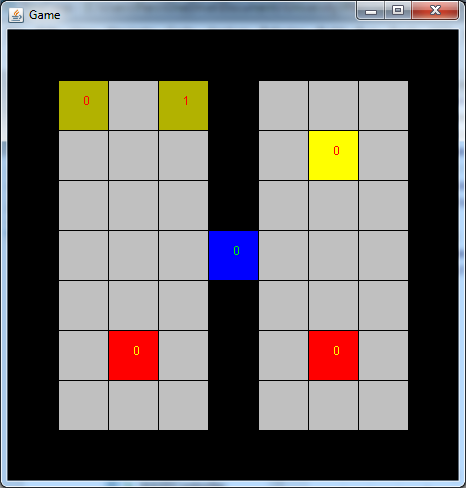
\includegraphics[scale=0.35]{InitialState}
\caption{Single Door \protect\footnotemark}
\label{SingleDoor}
\end{figure}
\footnotetext{Displayed numbers are the ID numbers - \emph{Button} ID 0 will open \emph{Door} ID 0 but not \emph{Door} ID 1}
\paragraph{\emph{Pathfinding}} This map is the same as \emph{SingleDoor} but without the \emph{Doors} and \emph{Buttons}. This was to test the \emph{Agent's} ability to solve the simplest problem.
\begin{figure}[H]
\centering
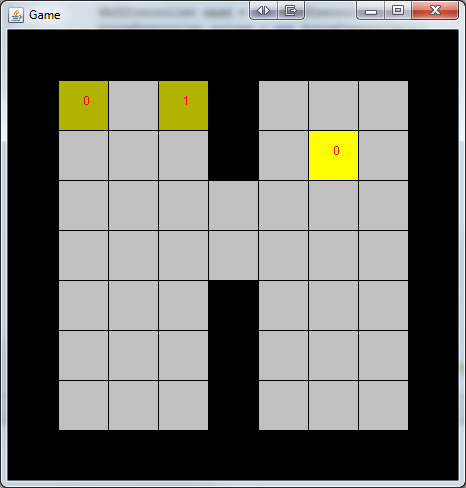
\includegraphics[scale=0.35]{level1e}
\caption{Pathfinding}
\label{Pathfinding}
\end{figure}
\paragraph{\emph{SymmetricSingleDoor}} This map was a modification of the \emph{SingleDoor} - making the map more symmetric and the action parts closer together.
\begin{figure}[H]
\centering
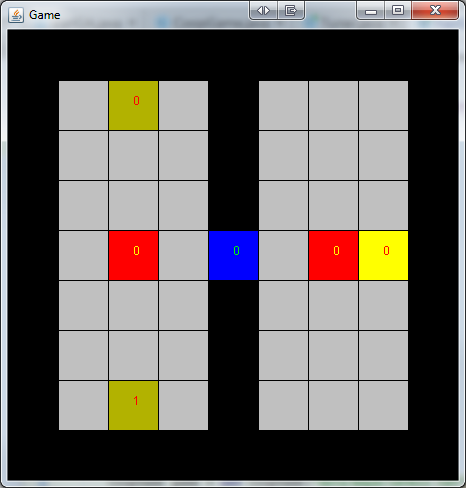
\includegraphics[scale=0.35]{level2}
\caption{Symmetric Single Door}
\label{SymmetricSingleDoor}
\end{figure}
\paragraph{\emph{ExtendedSide}} This map was an extension of \emph{SingleDoor} with a second \emph{Goal} and some extra walls in the game. Spreading the action parts away from the door and buttons was the main purpose of this one.
\begin{figure}[H]
\centering
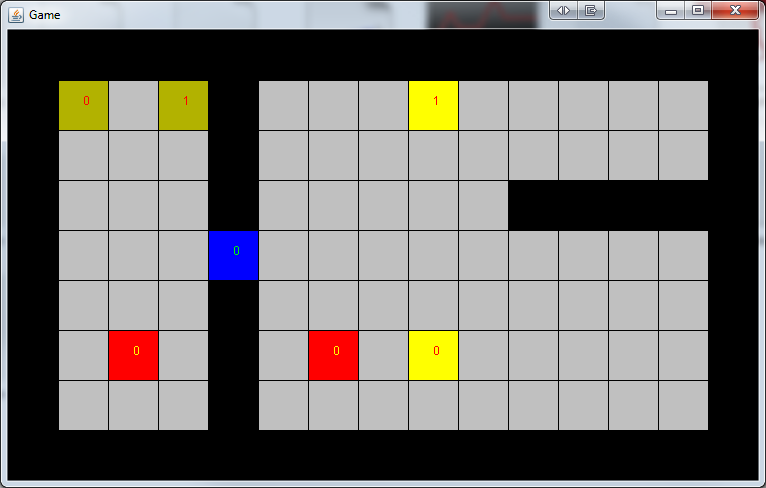
\includegraphics[scale=0.35]{level3}
\caption{Extended Side}
\label{ExtendedSide}
\end{figure}
\paragraph{\emph{SideBySide}} This map was a modification of \emph{SingleDoor} - putting a second \emph{Goal} in and making the map partly mirrored. Each \emph{Agent} began in a separate room to each other instead of together.
\begin{figure}[H]
\centering
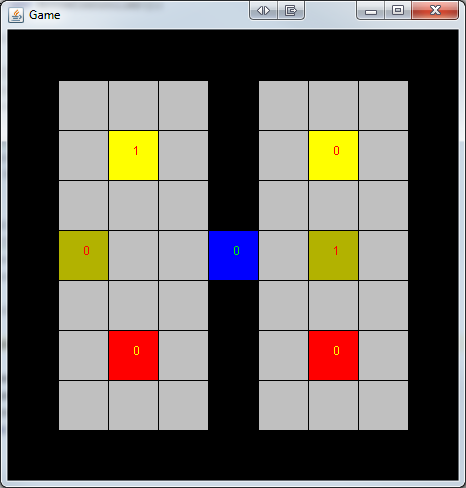
\includegraphics[scale=0.35]{level4}
\caption{Side By Side}
\label{SideBySide}
\end{figure}
\paragraph{\emph{Airlock}} This map was a new map, designed to give wildly different roles to each AI - the top Agent would have to travel through two doors (Like an airlock) that the bottom agent had access to the linked \emph{Buttons}. Then the top \emph{Agent} could collect the reward and allow the bottom \emph{Agent} access to the \emph{Goal}.
\begin{figure}[H]
\centering
\includegraphics[scale=0.35]{level5}
\caption{Airlock}
\label{Airlock}
\end{figure}
\paragraph{\emph{Butterfly}} This map was a new map - with two rooms each with a \emph{Goal} and a door. This was designed to force each \emph{Agent} to be let into the \emph{Goal} room, and out of it again.
\begin{figure}[H]
\centering
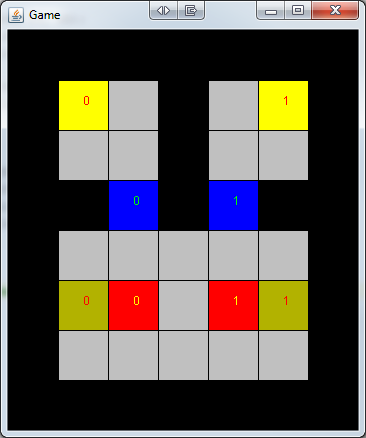
\includegraphics[scale=0.35]{level6}
\caption{Butterfly}
\label{Butterfly}
\end{figure}


\subsubsection{\gls{ai} Controllers}
A set of \gls{ai} Controllers were created in order to attempt to solve the problem domain. None of the agents have the ability to communicate with another agent and each agent has a single controller.
\paragraph{Random}
The random controller simply chooses one of the possible 5 actions. This is one of the simplest to implement and run.
\begin{comment}
\paragraph{Keyboard}
The keyboard controller takes input from the keyboard and translates that into a single Action. Once an action is polled, it is reset to the No Op action unless the keyboard is used again. 
\end{comment}
\paragraph{\gls{mcts}}
The \gls{mcts} controller is a simple implementation of \gls{uct} - with a fixed number of rollouts, \gls{uct} tree search depth limit and rollout border. The rollout border is how far in total, the forward model will be allowed to progress before the game is evaluated. No knowledge about the game is provided and the assumption is made that the other player will play randomly. The fixed rollout border makes a significant improvement in iterations per decision (from 1-3 to 500-600 in 40ms \footnote{Intel Core i5-3570, 8GB RAM, Windows 7 Enterprise 64bit}). This greatly improves the ability of \gls{mcts} to make informed decisions. The score at the end of a rollout is taken from the game state - so if \gls{mcts} does not see any player reach a goal, all branches will be equal.

For the tournament, three parameter sets were chosen for comparison and are shown in Table \ref{mctsTable}.
\begin{table}[!t]
\begin{center}
\begin{tabular}{|p{2.0cm}|p{2.0cm}|m{1.4cm}|m{1.4cm}|}
\hline
\textbf{Budget} & \textbf{Rollouts} & \textbf{UCT Search Limit} & \textbf{Rollout Border} \\
\hline
Small & 75 & 3 & 15 \\
Medium & 200 & 5 & 30 \\
High & 500 & 10 & 45 \\
\hline
\end{tabular}
\caption{Table of parameters for the 3 \gls{mcts} players}
\label{mctsTable}
\end{center}
\end{table}

\paragraph{Macro Action Genetic Algorithm}
The \gls{ga} algorithm was selected for its simplicity and had Macro Actions added in order to improve the forward search capability as well as the amount of computation time per decision available to it. The \gls{maga} used a population size of 10 and tournament selection of 3. Each candidate was a string of 15 actions - with each action performed 3 times in a row. This meant the \gls{maga} could "see" 45 ticks in the future. The design of the \gls{maga} algorithm was inspired by \textit{Perez et al} \cite{perez2013rolling}
\paragraph{Variable Macro Action Genetic Algorithm}
The Variable Macro Action \gls{ga} was created to try to solve the shortcomings of \gls{maga}. The primary premise was to allow the \gls{ga} to evolve the individual macro action lengths and the length of the overall sequence (number of macro actions). The main technique used was a 1 + 1 Evolutionary Strategy \cite{t.back2000evolutionary-co}. A 1 + 1 ES is a very simple \gls{ga} that maintains a single candidate, and in each iteration a mutation is made and if it is an improvement it is saved as the new best candidate. It is discarded if it is not an improvement. ES's are often much simpler than full \gls{ga} algorithms to create, often require much less memory and due to performing less within each iteration is able to use more of the available time budget than a full \gls{ga}. The algorithm was bounded by a number of parameters that are shown in Table \ref{vmagaTable}.
\begin{table}[!t]
\begin{center}
\begin{tabular}{| l | l | l |}
\hline
\textbf{Param} & \textbf{Controls} & \textbf{Value} \\
\hline
minNum & Number of Macro Actions & 3 \\
MaxNum & Number of Macro Actions & 10 \\
minLength & Length of Macro Actions & 1 \\
maxLength & Length of Macro Actions & 5 \\
numChance & Chance of altering Number & 0.25 \\
lengthChance & Chance of altering each length & 0.8 \\
actionChance & Chance of altering each action & 0.75 \\
\hline
\end{tabular}
\caption{Table of parameters for the Variable Macro Action Genetic Algorithm}
\label{vmagaTable}
\end{center}
\end{table}
These values need extensive tuning to realise the full potential of the algorithm and is a source of possible future work.
\section{Results}

\begin{figure}[!ht]
\centering
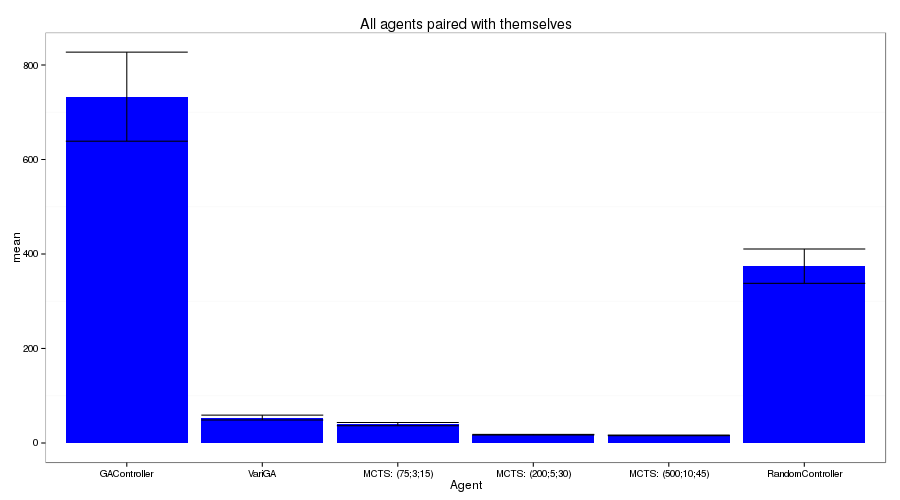
\includegraphics[width=\linewidth]{level1E-txt-pairs-ticks}
\caption{Average ticks taken to complete \emph{Pathfinding} when paired only with identical Agents}
\label{1epairedTicks}
\end{figure}

\begin{figure}[!ht]
\centering
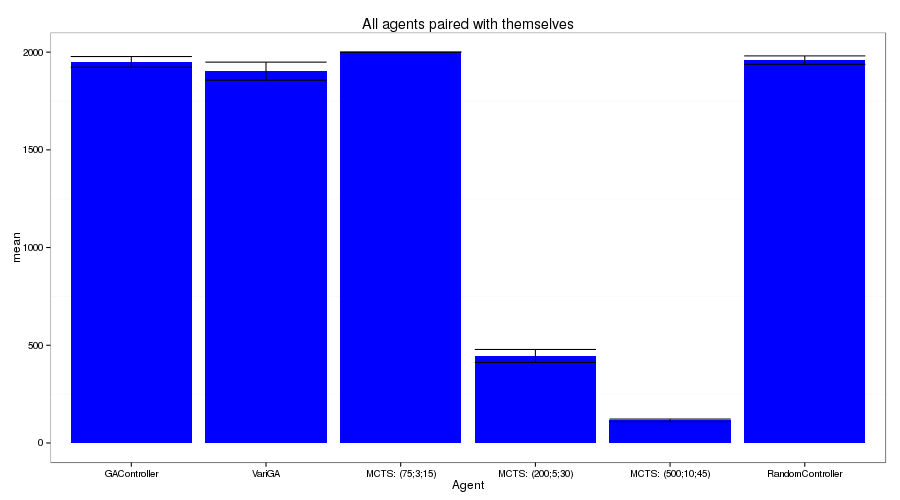
\includegraphics[width=\linewidth]{level1-txt-pairs-ticks}
\caption{Average ticks taken to complete \emph{SingleDoor} when paired only with identical Agents}
\label{1pairedTicks}
\end{figure}

Figure \ref{1epairedTicks} shows the ability of each Agent to solve a simple path finding problem. The \emph{GAcontroller}, with its macro actions, is hindered by its inability to make single step moves and has trouble actually walking straight to the target. The \emph{VariGA} does significantly better, due to its ability to perform single step moves. Figure \ref{1pairedTicks} shows that most of the controllers really struggle when the \emph{Door} and \emph{Buttons} are added. This indicates that the challenge of the task is high, although perhaps remarkable that \gls{mcts} is able to solve the task.

\begin{figure}[!ht]
\centering
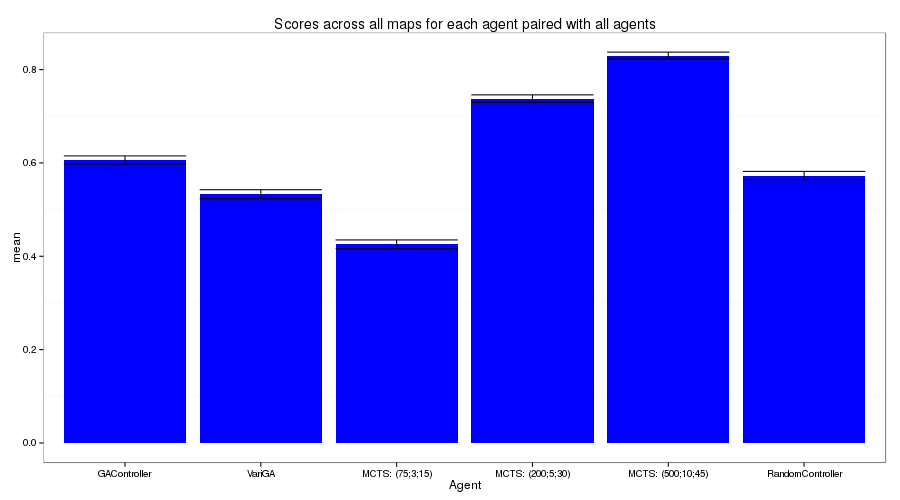
\includegraphics[width=\linewidth]{scores-allmaps}
\caption{Average score of each AI Agent over all pairings over all the Maps}
\label{avgScoreAllMaps}
\end{figure}

\begin{figure}[!ht]
\centering
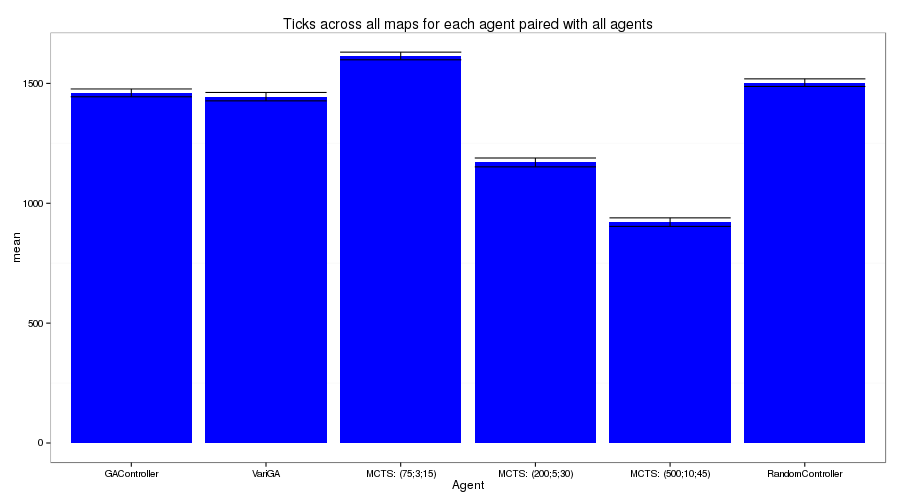
\includegraphics[width=\linewidth]{ticks-allmaps}
\caption{Average Ticks taken for each AI Agent over all pairings over all the Maps}
\label{avgTicksAllMaps}
\end{figure}

\begin{figure}[!ht]
\centering
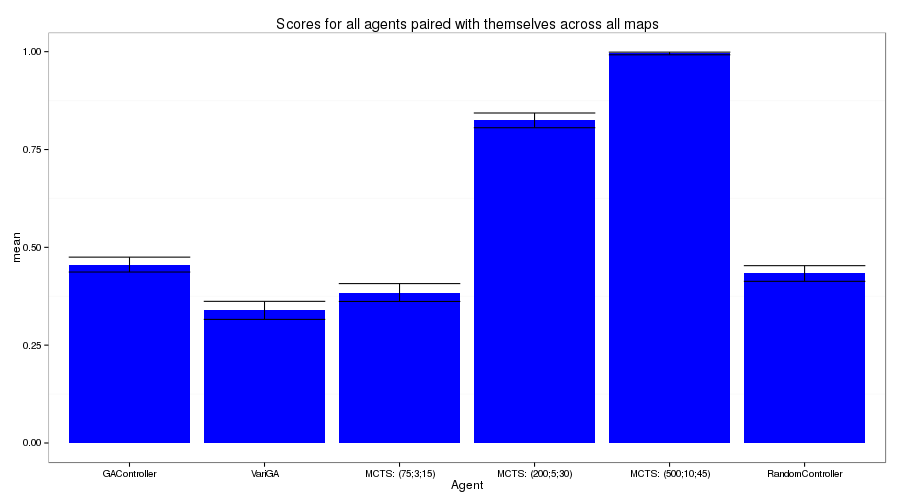
\includegraphics[width=\linewidth]{scores-samepairs}
\caption{Average Scores for each AI Agent paired with itself over all the Maps}
\label{avgScorePairAllMaps}
\end{figure}

\begin{figure}[!ht]
\centering
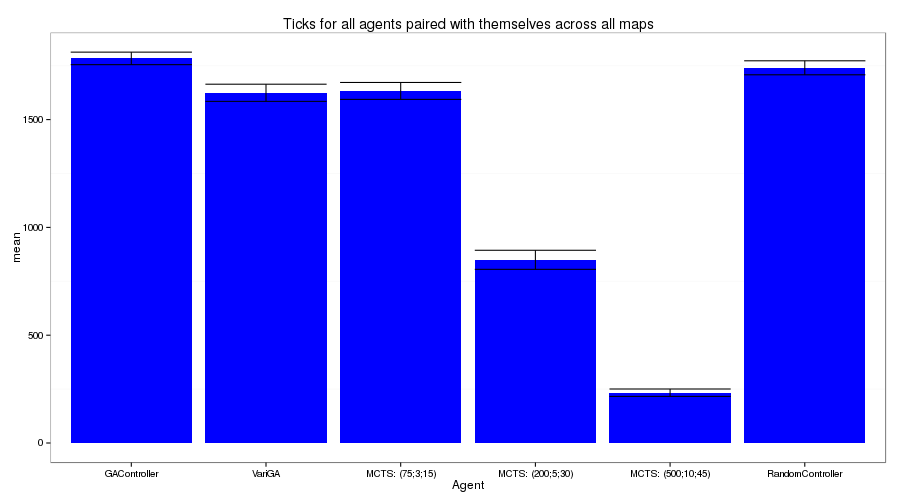
\includegraphics[width=\linewidth]{ticks-samepairs}
\caption{Average Ticks taken for each AI Agent paired with itself over all the Maps}
\label{avgTicksPairAllMaps}
\end{figure}

Figure \ref{avgScoreAllMaps} shows the average score that each AI Agent achieved over all the maps. The two more powerful \gls{mcts} Agents performed the best, doing much better than the competition. Figure \ref{avgTicksAllMaps} shows a similar result, with the more powerful Agents typically completing the maps in fewer ticks. \emph{RandomController} is the only deviant here - it outperformed the GA's in score but was worse in average ticks. Comparing the \gls{ai} \emph{Agents} when paired only with themselves in Figure \ref{avgScorePairAllMaps} and Figure \ref{avgTicksPairAllMaps}. The good results for \emph{RandomController} are potentially due to the fact that the 3 \gls{mcts} controllers and 2 \gls{ga} algorithms all based their decisions on having Random as an accomplice.

\begin{figure}[!ht]
\centering
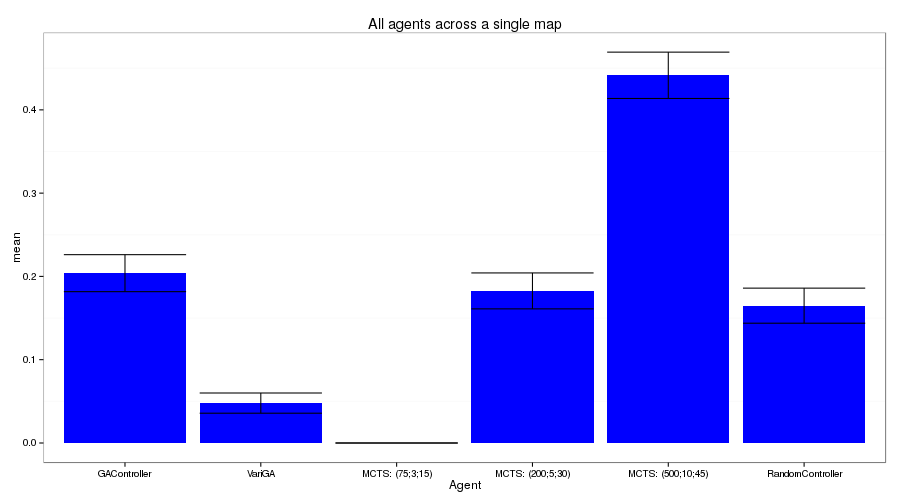
\includegraphics[width = \linewidth]{level5-txt-scores}
\caption{Average Score for each AI Agent paired with itself over \emph{Airlock}}
\label{avgScoreMap5}
\end{figure}

Airlock - shown in Figure \ref{Airlock} - poses a particular problem for many of the agents (see Figure \ref{avgScoreMap5}). The asymmetric nature of the level, and the delayed reward caused great difficulty for the Agents. Relying on two button presses and the other agent to get through the open doors - in order - greatly reduced performance. The top agent, \emph{High MCTS}, only managed an average score of $0.44$ compared to its total average of just over $0.8$.

\section{Discussion}
\subsection{MCTS}
\gls{mcts} performed very well in this problem domain. 

As seen above, in Figure \ref{avgTicksPairAllMaps}, the medium and high budget implementations provided the two quickest completion times across all maps. The differences shown were significant as well as being the only two agents to complete on average in under 1000 ticks.  Figure \ref{avgScorePairAllMaps} showed that the medium and high budget implementations scored significantly better than all other agents.

One possible reason for \gls{mcts} scoring so well in this problem domain is its use of statistics over hundreds and thousands of simulations to provide it with the ability to act in such a way that it handles all eventualities. Statistically,  in certain situations \gls{mcts} would only see rewards in the tree when it was situated on a \emph{Button}. This tended to cause the \gls{mcts} to travle towards \emph{Buttons}, increasing the likelihood that its own simulations would cause it to be situated on the button. Eventually, most other \gls{ai} \emph{Agents} would cross through the open door.
\subsection{GA}
The two \gls{ga} algorithms did not perform very well in this problem domain. 

As seen in Figure \ref{avgScorePairAllMaps} and Figure \ref{avgTicksPairAllMaps}, when tasked with solving the problem domain with another identical agent, neither the \emph{GAController} or \emph{VariGA} performed well at all. The \emph{VariGA} only performed significantly better than either \emph{RandomController} or \emph{GAController} in \emph{Pathfinding}. In all other cases, \emph{VariGA} performed similarly to the standard \emph{GAController}. The ability to mutate the lengths of individual action sequences made the \emph{VariGA} a more flexible pathfinder that the \emph{GAController} but did not aid its ability to solve the co-operative problems present elsewhere in the experiment.

The \gls{ga} algorithms do not have the stored tree structure of \gls{mcts} with which to gain the statistical model for what happens when they pursue certain actions. This leads to a seemingly poor performance for the \gls{ga} despite \gls{ga} and \gls{mcts} typically performing equally well in other domains.
\subsection{Random}
The \emph{RandomController} performed poorly in this problem domain. On average, the \emph{RandomController} finished under the 2000 tick limit and scored less than half the maximum on average.
\section{Conclusions}
In this paper, we found that a strong MCTS player can solve simple cooperative problems without requiring communication between agents. We also found that a number of other \gls{ai} techniques experienced difficulty when the problem became cooperative. Further work is required in this area.

\subsection{Further Work}
There is scope for more work in a number of areas.

\subsubsection{Communication}
More work can be conducted in the writing of AI's to use communication in order to complete these challenges better amongst themselves. A framework for communication would be devised - with the requirement for fairly \gls{ggp} like restrictions in mind. Use of the communication framework would need to likely be learned by the \emph{Agents} during play, posing a particular challenge for the future.

\subsubsection{Optimisations}
Future work should also include some work to ensure that the \gls{ai} Agents have their parameters set correctly. The \emph{High MCTS} performed well - showing the power of having the correct parameters compared to the \emph{Low MCTS}. The \emph{VariGA} has 7 parameters that we simply did not have time to correctly optimise for this experiment.

\subsubsection{Problem Domain}
More work can also be done on experimenting with the problem domain itself. Expanding the object types to include different techniques such as pickup-able objects that can be placed on \emph{Buttons}, \emph{Buttons} that remain active for a period of time after vacating them as well as potentially \emph{Doors} that will open permanently if all it's \emph{Buttons} are activated. The scope here is fairly limitless.

\bibliographystyle{IEEEtran}
\bibliography{ceec}

\end{document}